\documentclass[a4paper,11pt]{article}
\usepackage{pos}

\usepackage{caption}
\usepackage{float}
\usepackage[lofdepth=1,lotdepth]{subfig}

\usepackage{braket}

\usepackage[noabbrev, capitalise, nameinlink]{cleveref}  % reference object types automatically

% until reviewed
\usepackage{lineno}
\linenumbers

\title{Search for heavy neutral lepton production and decay with the IceCube Neutrino Observatory}
\ShortTitle{Search for heavy neutral lepton production and decay with IceCube}

\manuallySeparateAuthors
\author*[a]{Leander Fischer}
% \author[b]{and Julia Book}
\author{for the IceCube collaboration}

\affiliation[a]{DESY, D-15738 Zeuthen, Germany}
% \affiliation[b]{Harvard University, Cambridge, MA 02138, USA}

\emailAdd{leander.fischer@desy.de}
% \emailAdd{jbook@g.harvard.edu}

\abstract{
Sterile neutrinos are a well motivated objective of Beyond Standard Model searches. Extensions to the Standard Model including right handed (sterile) neutrinos pose a viable explanations for the origin of neutrino masses and they could also solve a variety of additional open questions in physics such as neutrino oscillation anomalies, the nature of dark matter, and baryon asymmetry. Multiple models posit the existence of a GeV-scale, sterile neutrino (also called heavy neutral lepton), which can interact with the Standard Model particles through kinetic mixing. The heavy neutral lepton can therefore be produced from and decay into the known particles. If the production from atmospheric neutrino up-scattering and the heavy neutral leptons subsequent decay happen inside the IceCube detector, it can produce a unique double-cascade signature, which can be utilized to search for GeV-scale heavy neutral leptons at atmospheric neutrino energies. Focusing on the flux of atmospheric muon neutrinos that oscillate into tau neutrinos, the less constrained $\tau$-sterile mixing space can be explored. We present the initial analysis approach of studying heavy neutral leptons in the mass range of 0.1-3 GeV, by searching for low-energy double-cascade topologies with the IceCube DeepCore detector, as well as the difficulties of this search and the resulting necessary restructuring of the analysis approach.
}

\FullConference{
  41st International Conference on High Energy physics - ICHEP2022\\
  6-13 July, 2022\\
  Bologna, Italy
}

\begin{document}
\maketitle


\section{Introduction}

Extensions to the Standard Model (SM) adding heavy neutral leptons (HNLs) provide a good explanation to the origin of neutrinos masses through type-I seesaw mechanisms \cite{10.1143/PTP.64.1103}. While the mixing with $\nu_{e/\mu}$ is strongly constrained ($|U_{\alpha4}^2| \lesssim 10^{-5}-10^{-8}, \alpha=e,\mu$), the mixing with $\nu_{\tau}$ is much harder to probe, due to the difficulty of producing and detecting tau neutrinos. \cref{fig:hnl_limits_and_decay_widths} (left) shows the current limits on the $\tau$-sterile mixing for HNL masses between $0.1-10$\,GeV. As was first pointed out in \cite{Coloma:2017ppo}, the atmospheric neutrino flux observed in IceCube offers offer a way to constrain the neutrino-HNL mixing parameters. Using the large fraction of atmospheric $\nu_{\mu}$ events that oscillate into $\nu_{\tau}$ until they reach the detector \cite{IceCube:2019dqi}, the less constrained $\tau$-sterile mixing space can be explored.

\begin{figure}[h]
  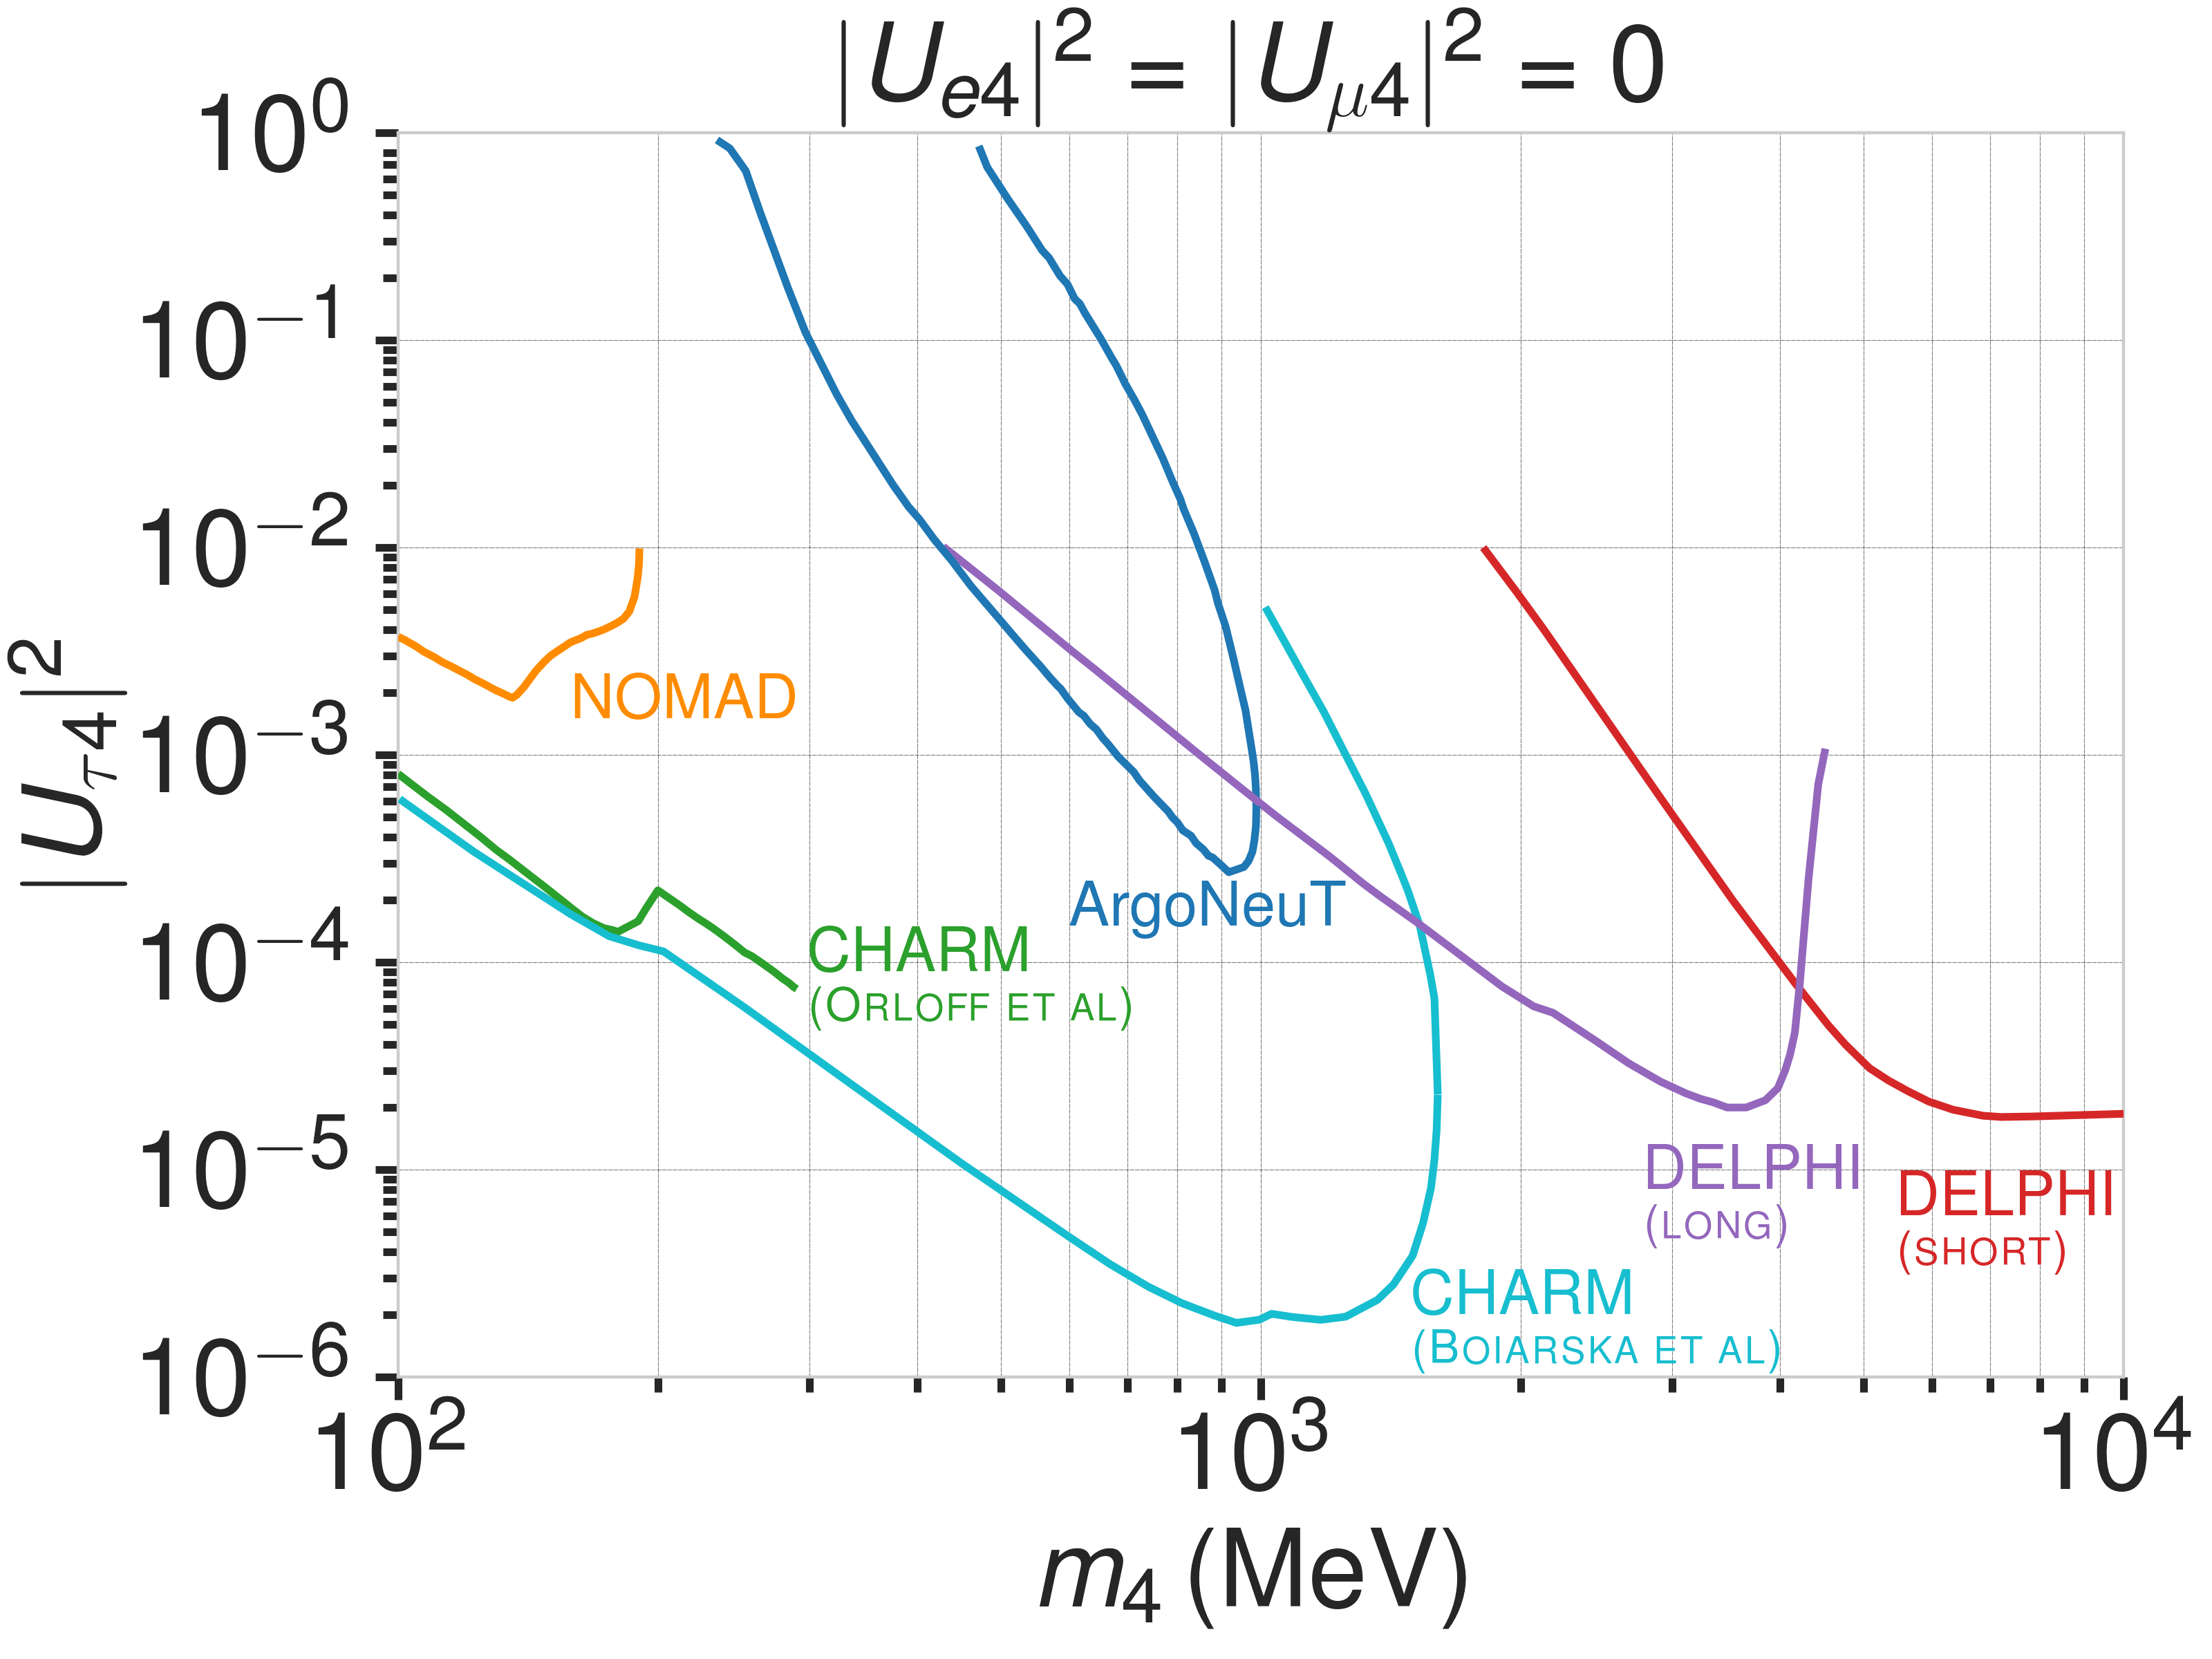
\includegraphics[width=.50\linewidth]{figures/UtauN_custom_plots_LF_grid_white.png}
  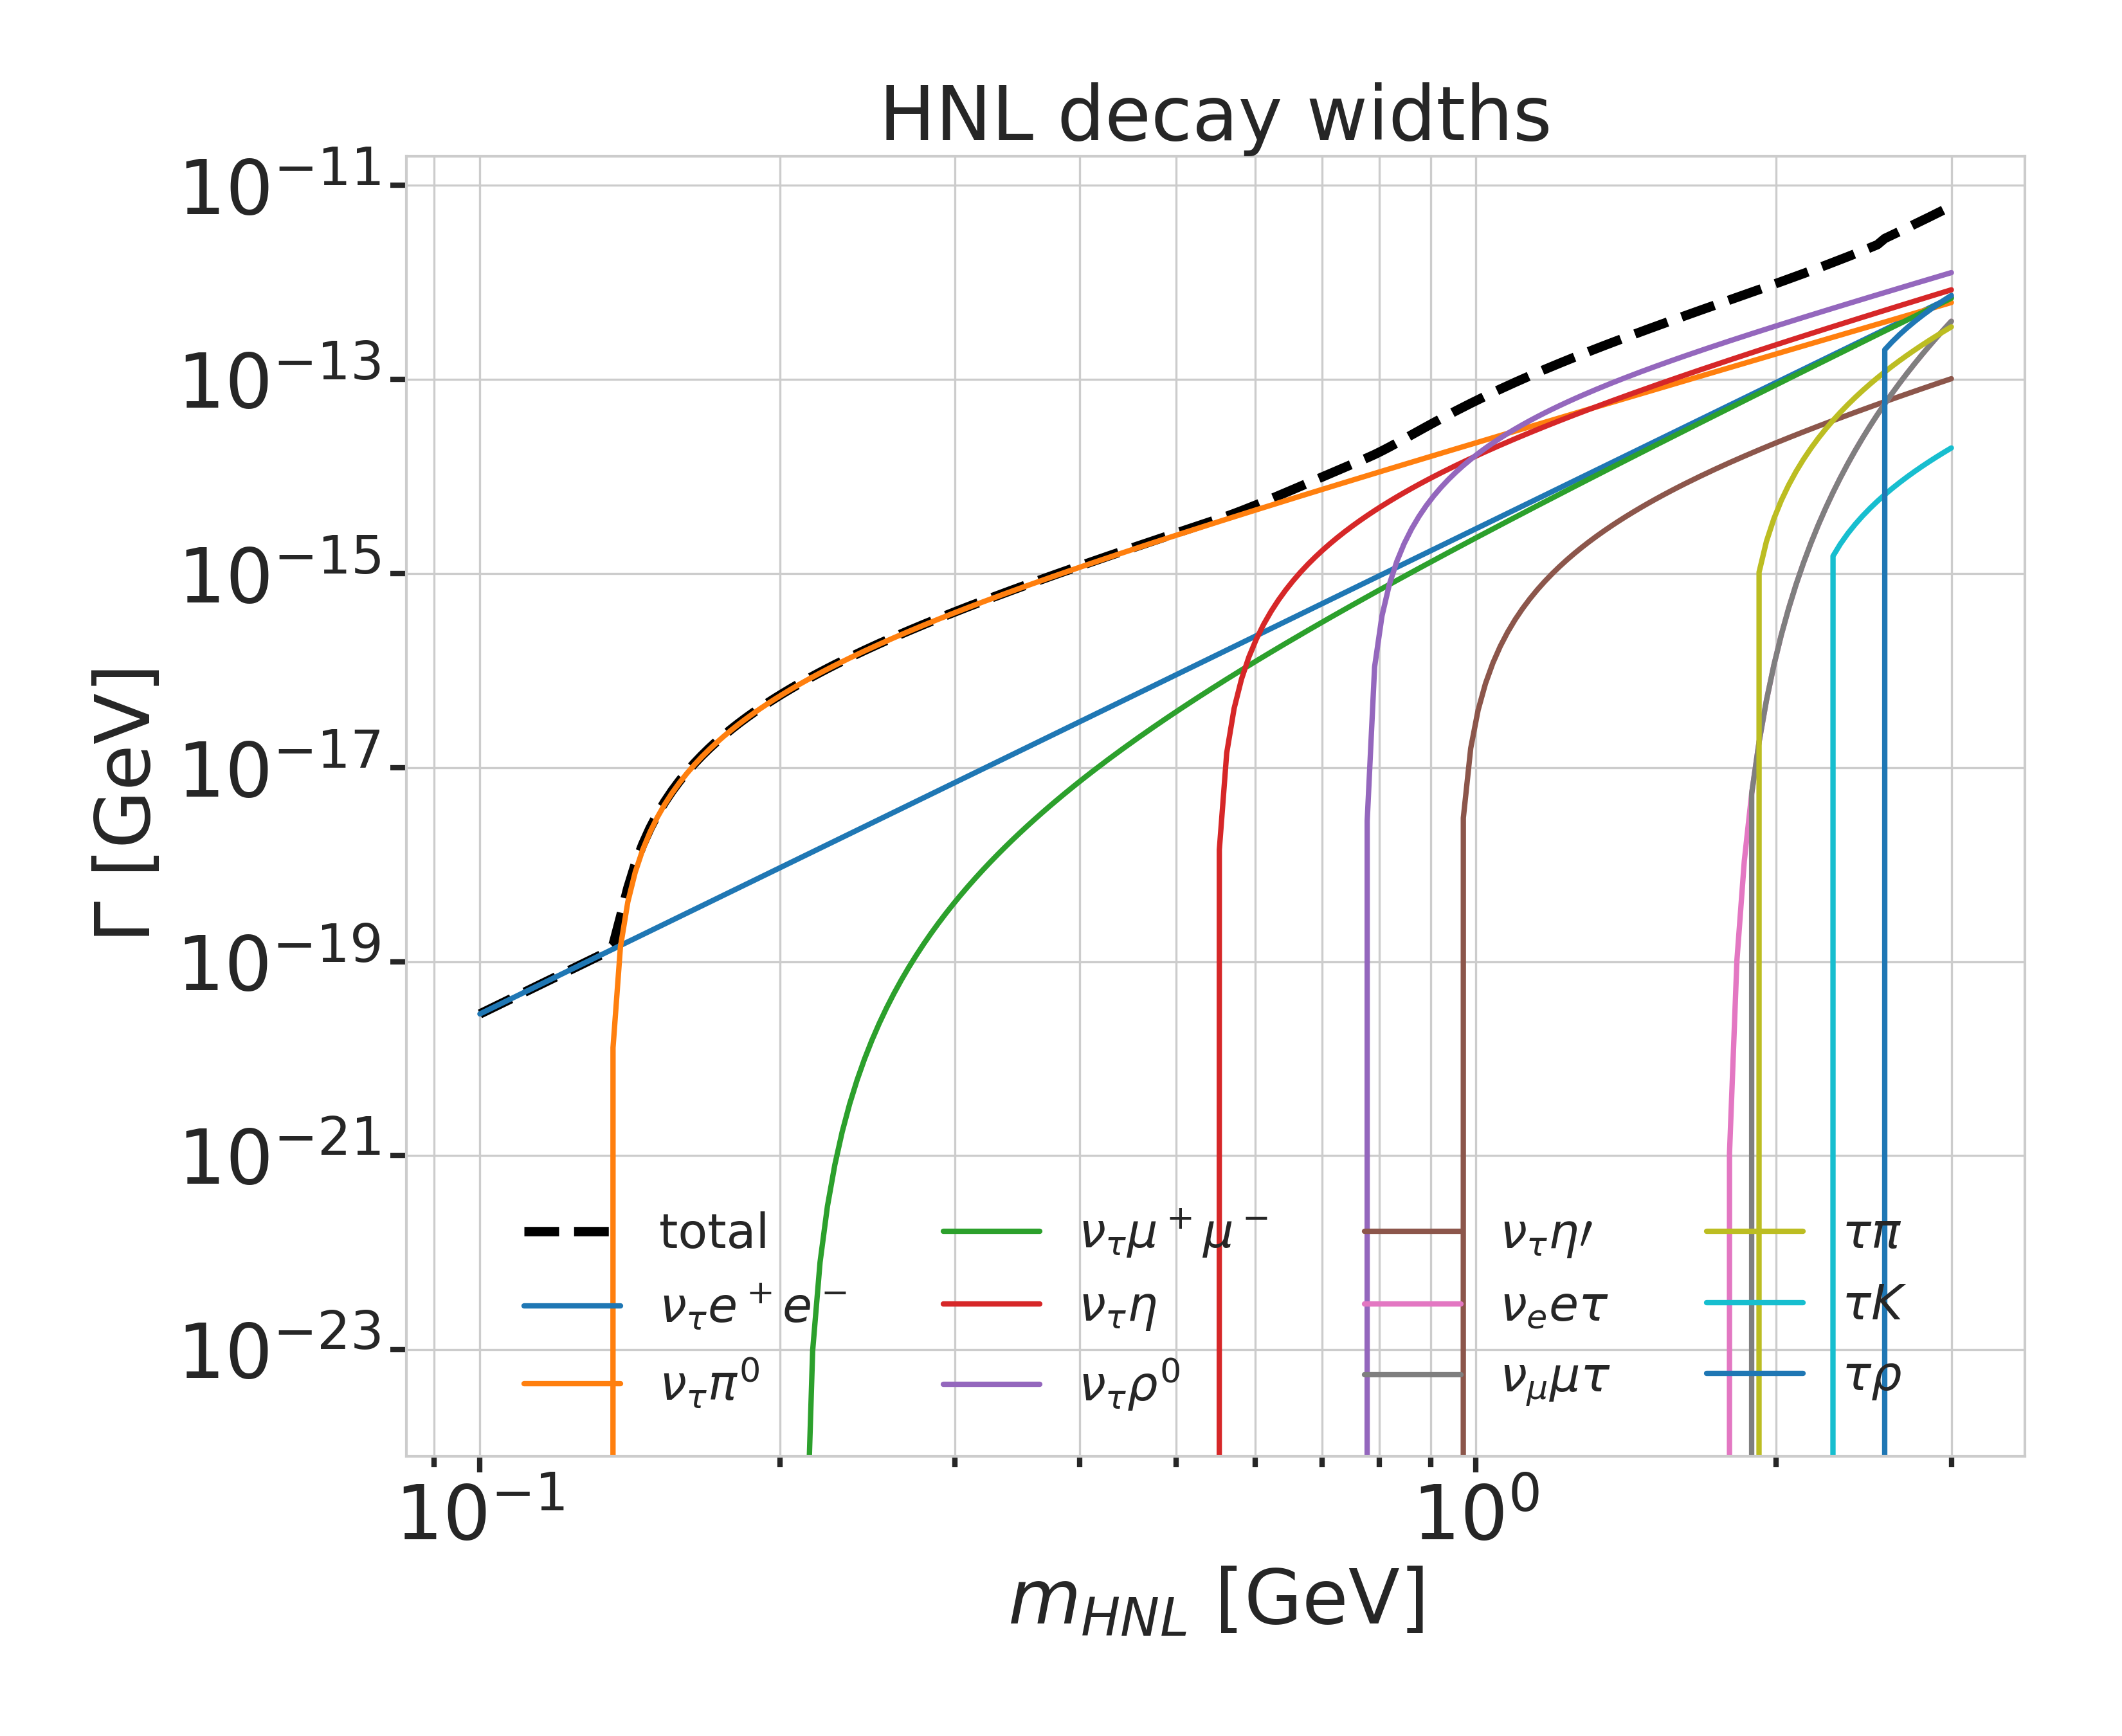
\includegraphics[width=.47\linewidth]{figures/hnl_decay_widths_log.png}
  \label{fig:hnl_visible_decay_widths}
  \caption{Current $|U_{\tau4}^2|$ limits (left) from NOMAD \cite{NOMAD:2001eyx}, ArgoNeut \cite{ArgoNeuT:2021clc}, CHARM \cite{Orloff:2002de, Boiarska:2021yho}, and DELPHI \cite{DELPHI:1996qcc} and decay widths of visible decay modes in IceCube (right) calculated based on the results from \cite{Gorbunov:2007ak}.}
  \label{fig:hnl_limits_and_decay_widths}
\end{figure}


\vspace{-0.75cm}
\section{IceCube DeepCore}

\begin{figure}[h!]
  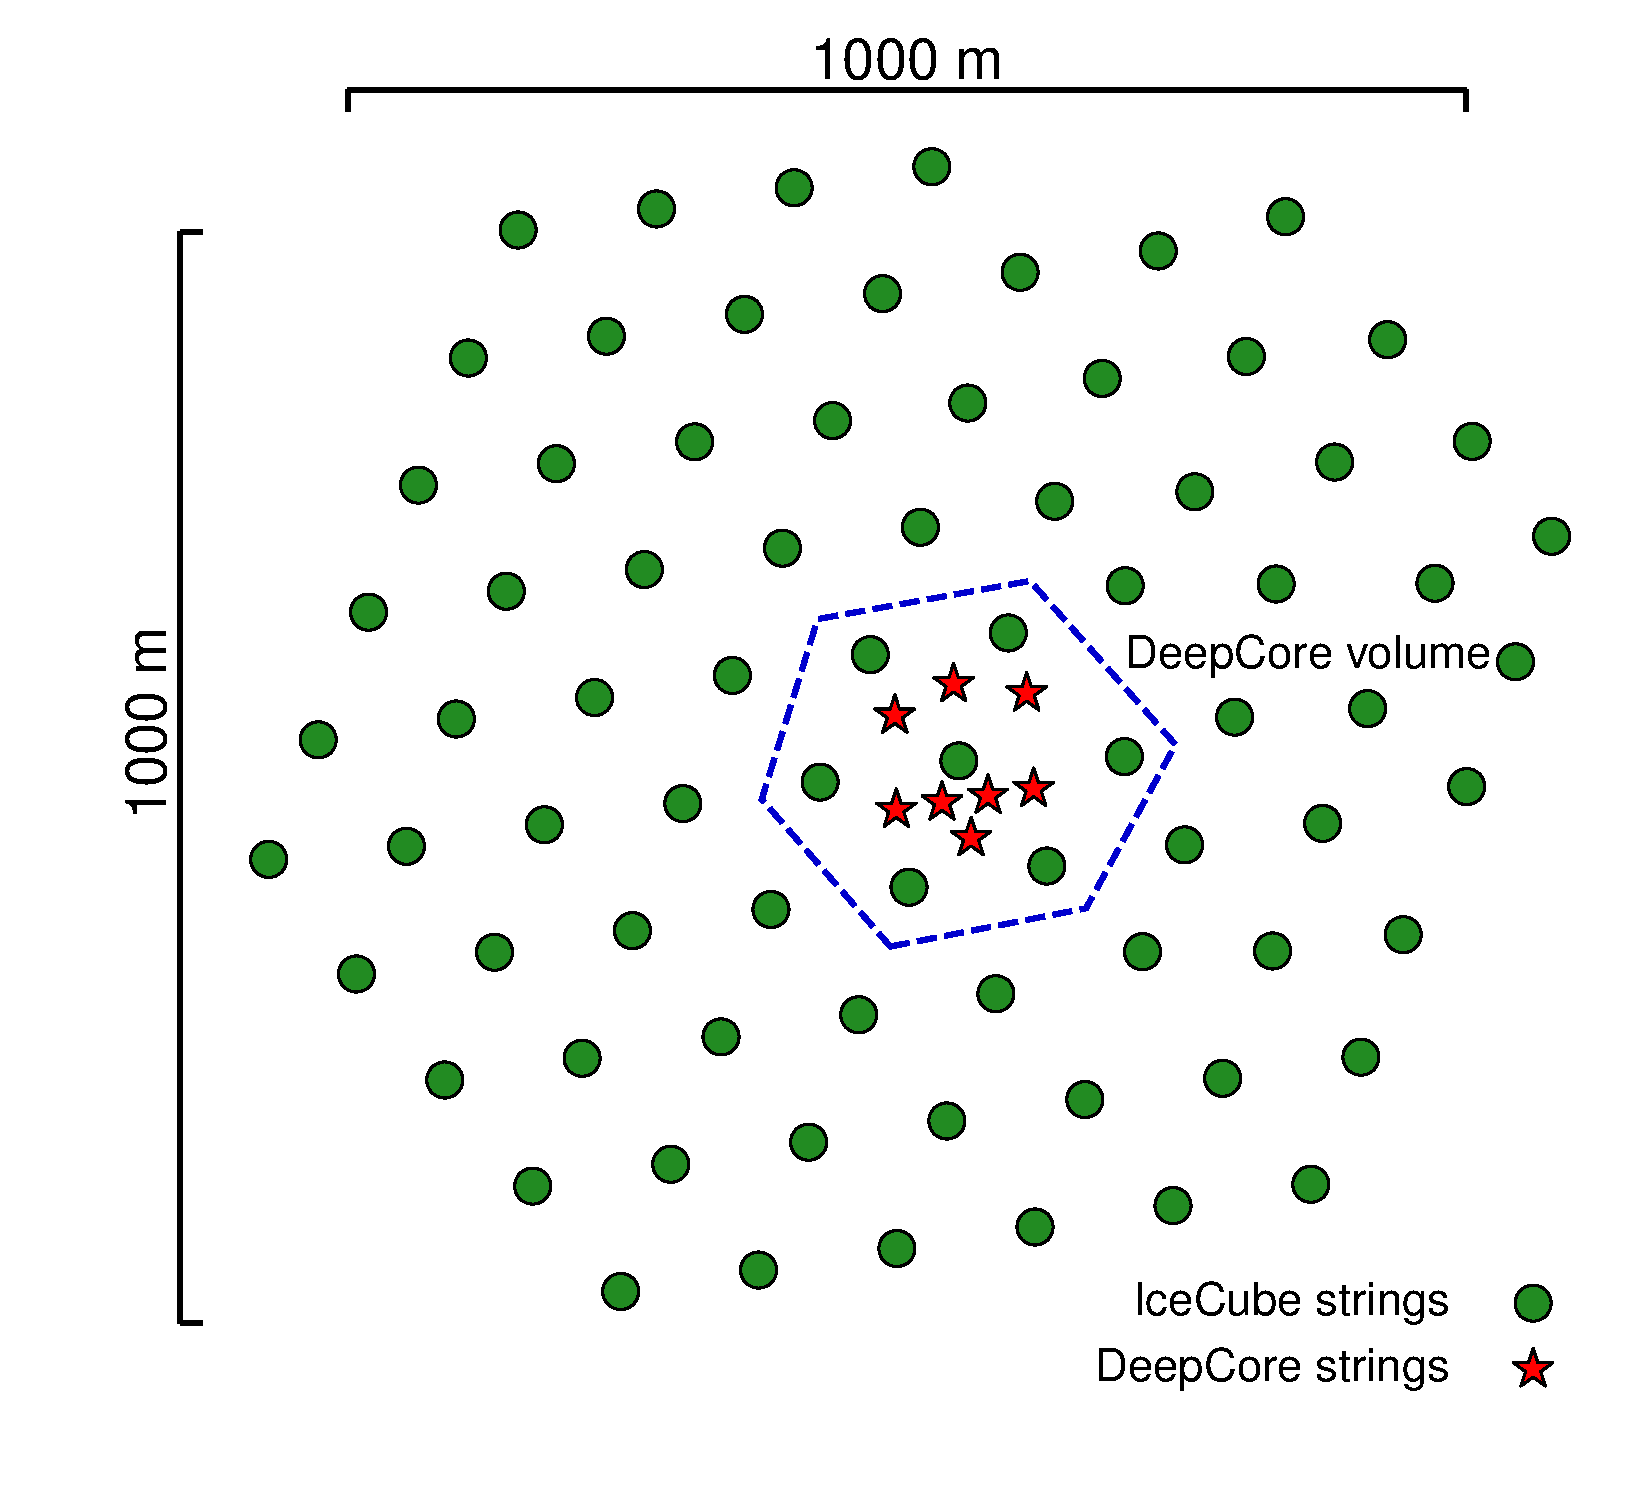
\includegraphics[width=.43\linewidth]{figures/icecube_top_view_bw.pdf}
  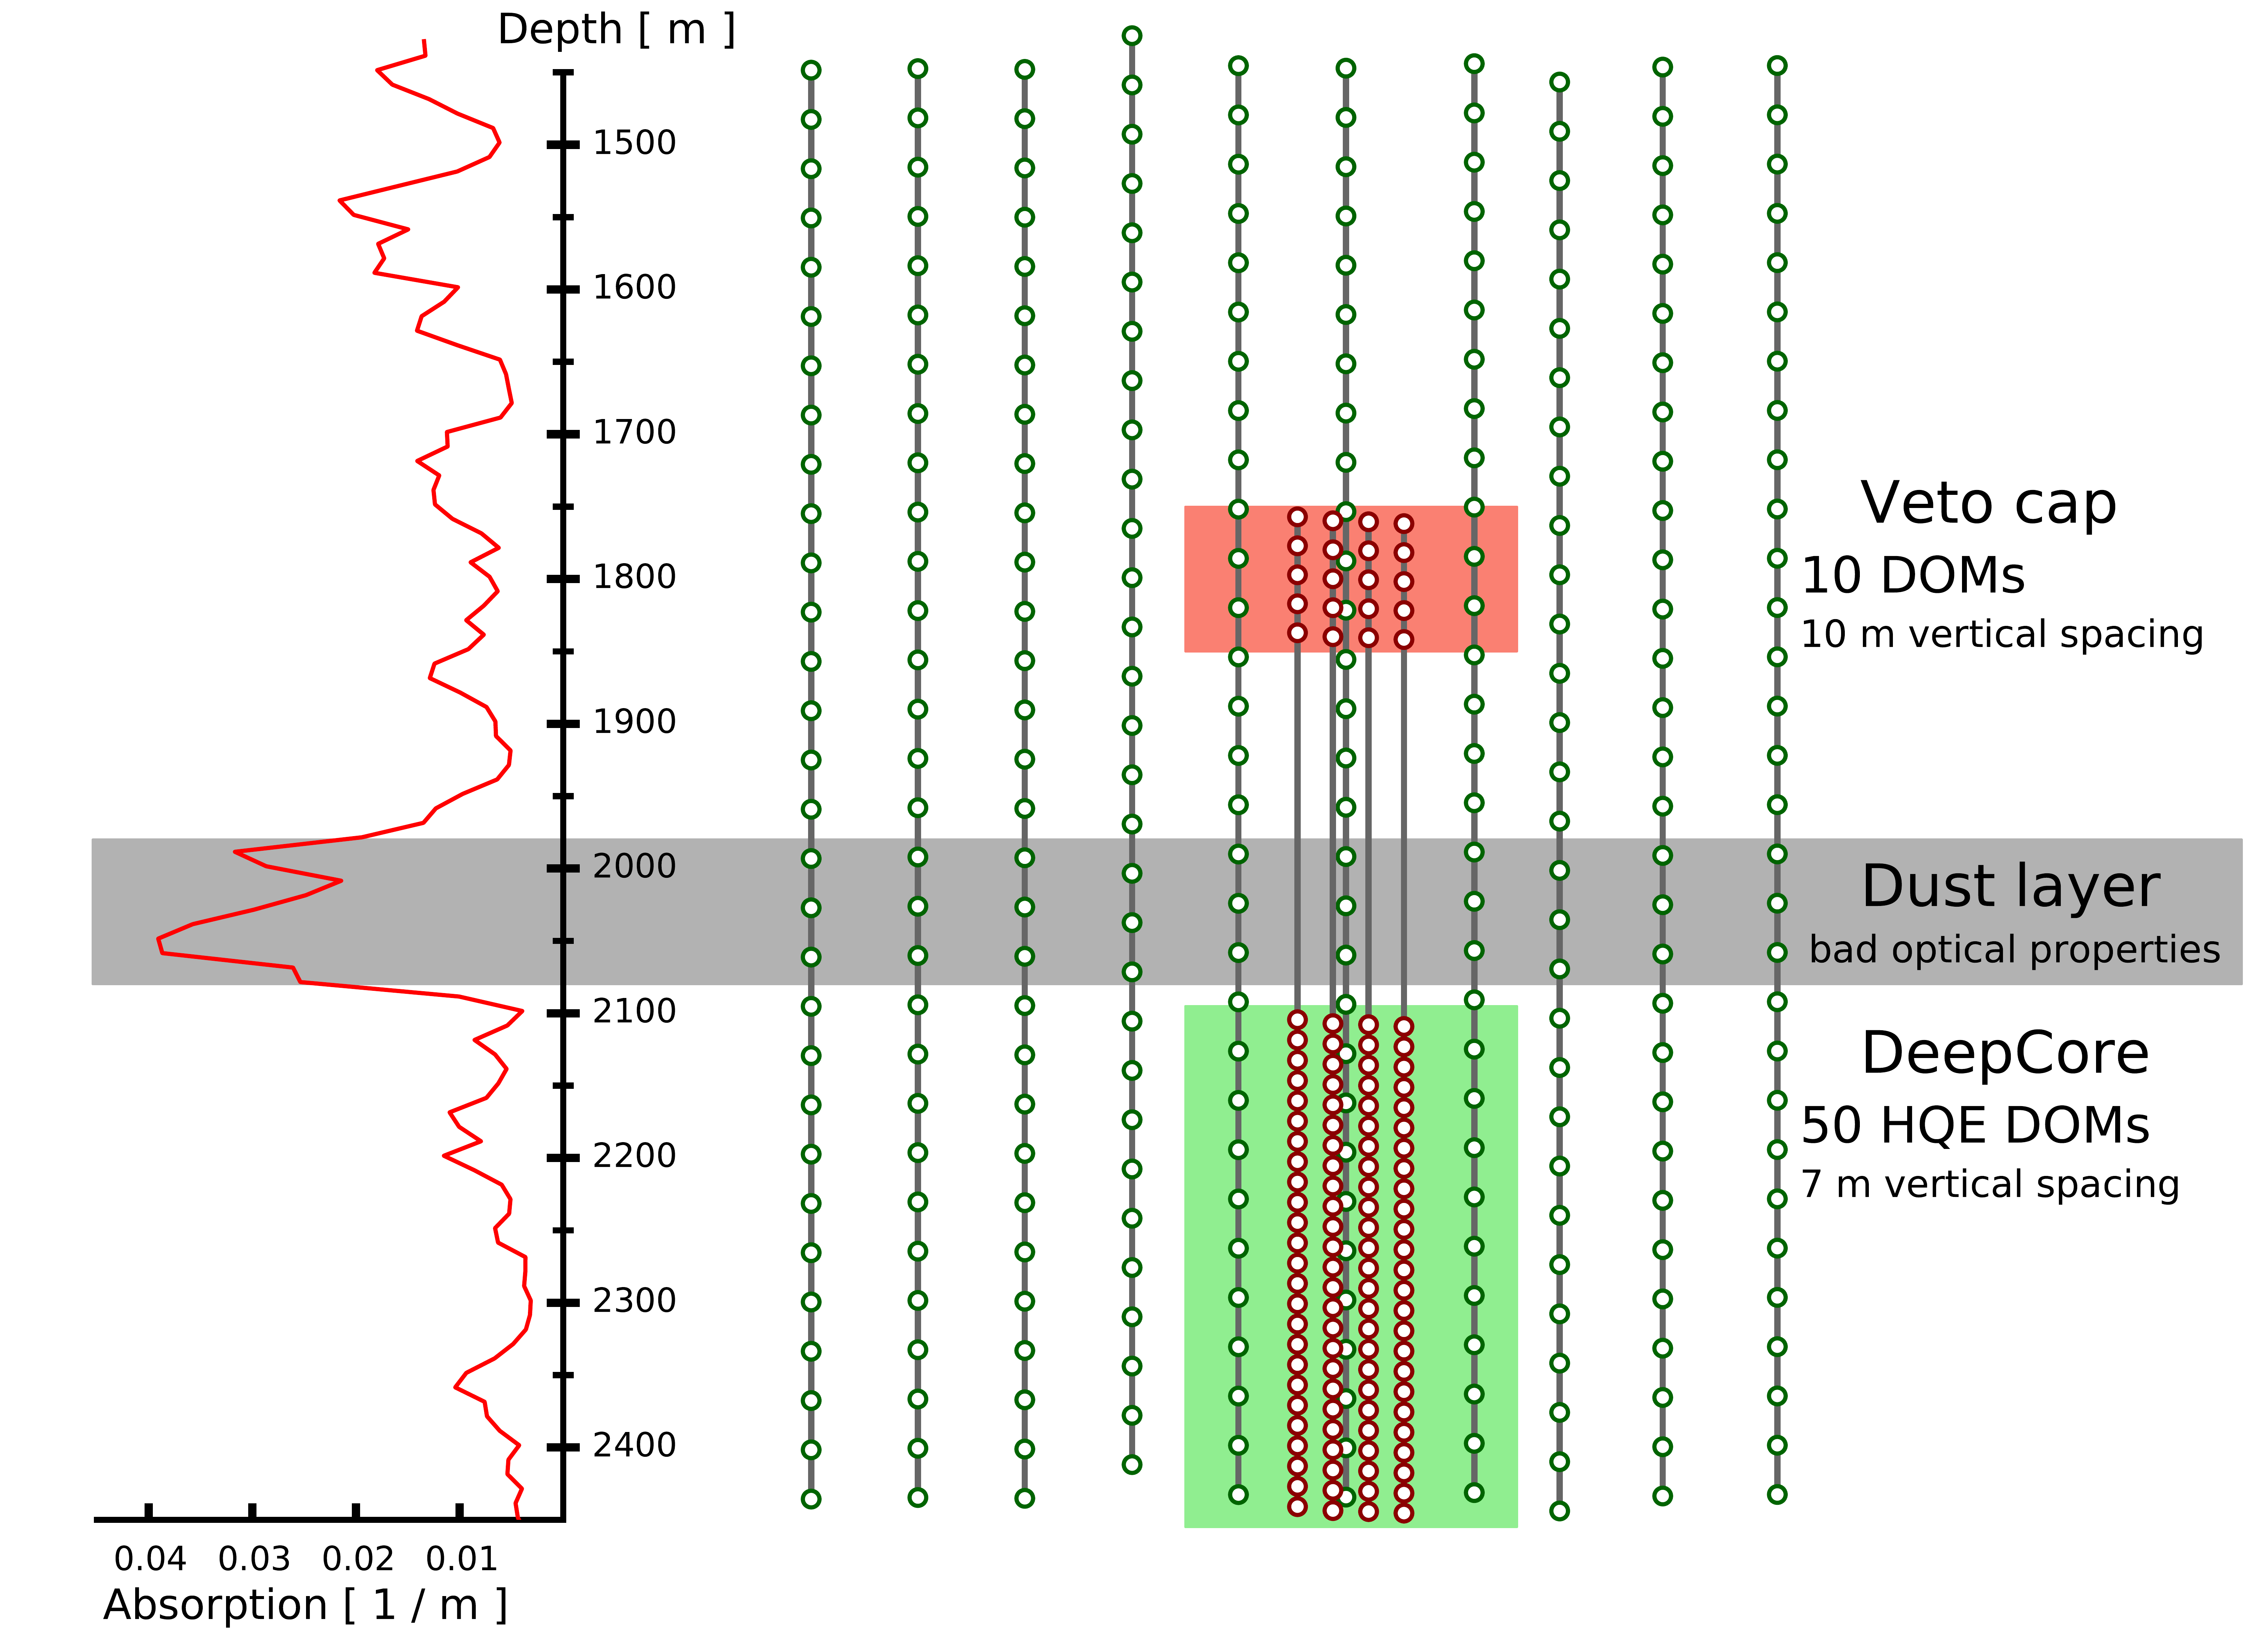
\includegraphics[width=.52\linewidth]{figures/DeepCore_sideview.png}
  \caption{Top-view (left) and side-view (right) of the IceCube and DeepCore array. The side-view also shows the ice absorption at different depths.}
  \label{fig:icecube_array}
\end{figure}

The IceCube Neutrino Observatory \cite{Aartsen:2016nxy} is located at the geographic South Pole and consists of 5160 Digital Optical Modules (DOMs), deployed into the antarctic glacial ice at depths between 1.45\,km and 2.45\,km. It is an ice Cherenkov telescope instrumenting a volume of about 1\,km$^{3}$. The ice is used as interaction and detection medium, simultaneously, where interacting neutrinos can produce charged secondary particles, which themselves can emit Cherenkov photons detectable by the DOMs. The DOMs are arranged on a nearly-hexagonal array, as shown in \cref{fig:icecube_array}, with 125\,m horizontal and 17\,m vertical spacing in IceCube and a closer 42-72\,m horizontal and 7\,m vertical spacing in the denser, bottom-center part of the array, called DeepCore \cite{IceCube:2011ucd}. While IceCube targets the detection of astrophysical neutrinos with energies above $\sim$100\,GeV, DeepCore can measure neutrino interactions down to a few GeV, due to its closer spacing in regions with very good optical properties of the ice. The location of DeepCore is indicated in \cref{fig:icecube_array} (left/right), which also shows the absorption properties of the ice with respect to depth (right).

\begin{figure}[h!]
    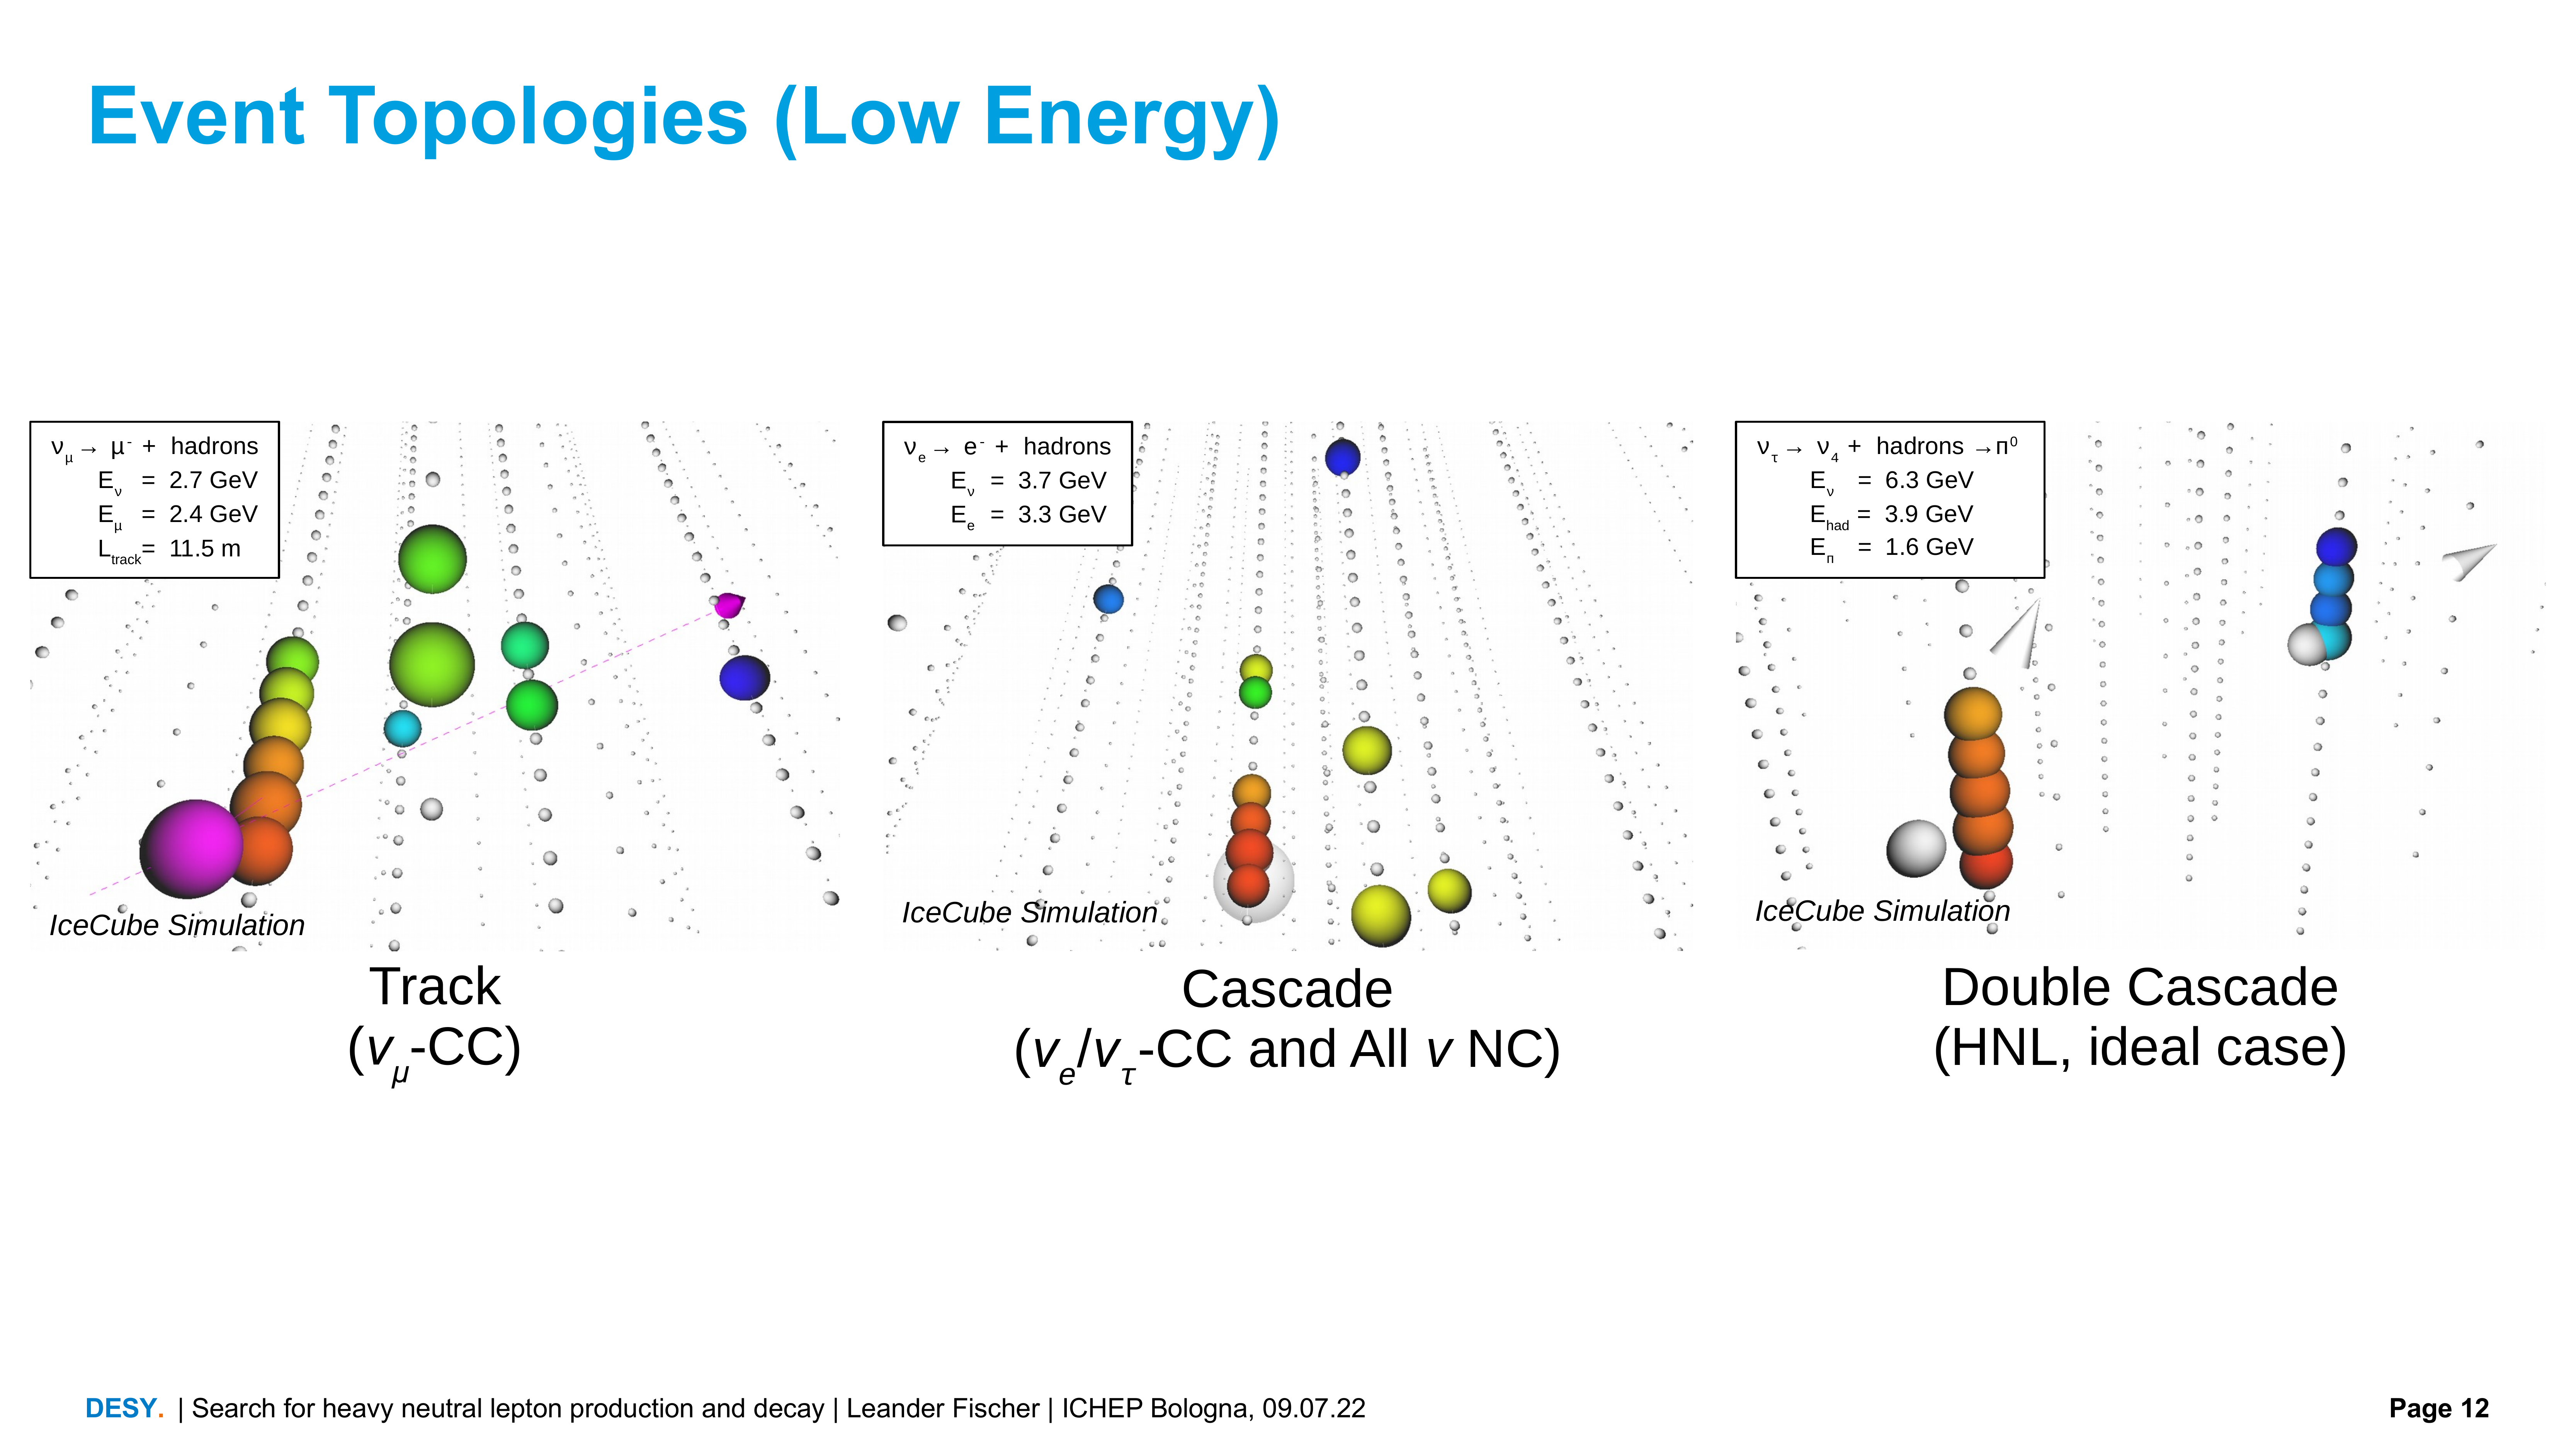
\includegraphics[trim = 0cm 4.5cm 0cm 5.5cm, clip, width=1.0\linewidth]{figures/event_views_all_three.png}
    \caption{Example of low energy event topologies in IceCube DeepCore. The color of the spheres indicates the arrival time of the photons while its size is relative to the number of photons that were detected.}
    \label{fig:low_energy_eventviews}
  \end{figure}

The two observable low energy event topologies in IceCube DeepCore are \textit{tracks} and \textit{cascades}. Tracks are elongated light emission patterns, produced by long-lived muons, mainly originating from $\nu_{\mu}$ charged current (CC) interactions or cosmic ray air showers, with a subdominant component from $\nu_{\tau}$ CC interactions (BR of $\tau\rightarrow\mu$ $\sim17\,\%$ \cite{PhysRevD.98.030001}). Cascades are roughly point-like, spherical light emissions, produced by electromagnetic and hadronic showers. They are produced by $\nu_{e}$ CC and most $\nu_{\tau}$ CC interactions, as well as neutral current (NC) interactions of all flavours. \cref{fig:low_energy_eventviews} left and middle show examples of track-like and cascade-like topologies at atmospheric energies. The main measurement performed with IceCube DeepCore is a measurement of atmospheric neutrino oscillation parameters.


\vspace{-0.5cm}
\section{Neutrino Oscillations} \label{sec:neutrino_oscillations}

Neutrino wave functions can be described by their mass eigenstates or their flavor eigenstates \cite{BILENKY1978225}, which are related as $\ket{\nu_\alpha} = \sum_kU^{3x3*}_{\alpha k}\ket{\nu_k}$, where $\ket{\nu_\alpha}$ are the flavor states with $\alpha=e,\mu,\tau$ and $\ket{\nu_k}$ the mass states with $k=1,2,3$. $U^{3x3}_{\alpha k}$ is the Pontecorvo-Maki-Nakagawa-Sakata (PMNS) matrix defining the mixing between mass and flavor states. The flavor states, which therefore are a superposition of the mass states \cite{PhysRevD.98.030001}, link the neutrinos to the charged leptons they interact with in weak CC interactions. A neutrino, produced in its flavor state, will propagate through space as its composing mass states. For (at least two) nonzero, non-equal neutrino masses, this leads to the observed phenomenon of neutrino oscillations, meaning that the neutrino changes from its initial flavor to another flavor and back after traveling a certain distance.

\begin{figure}[h!]
  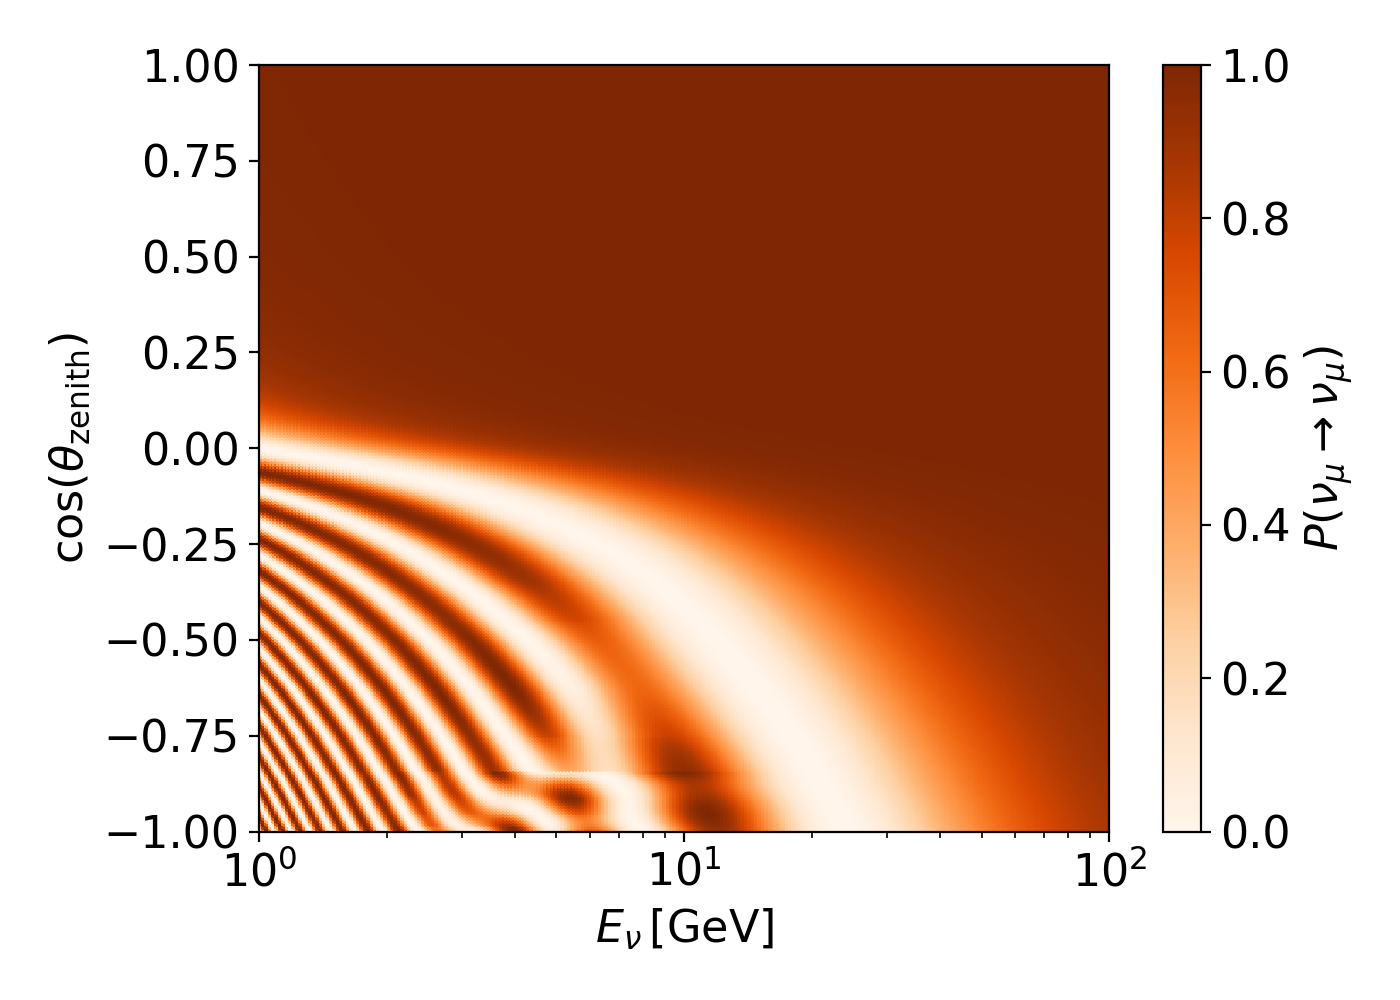
\includegraphics[width=.44\linewidth]{figures/Oscillogram_numu_numu_orange.png}
  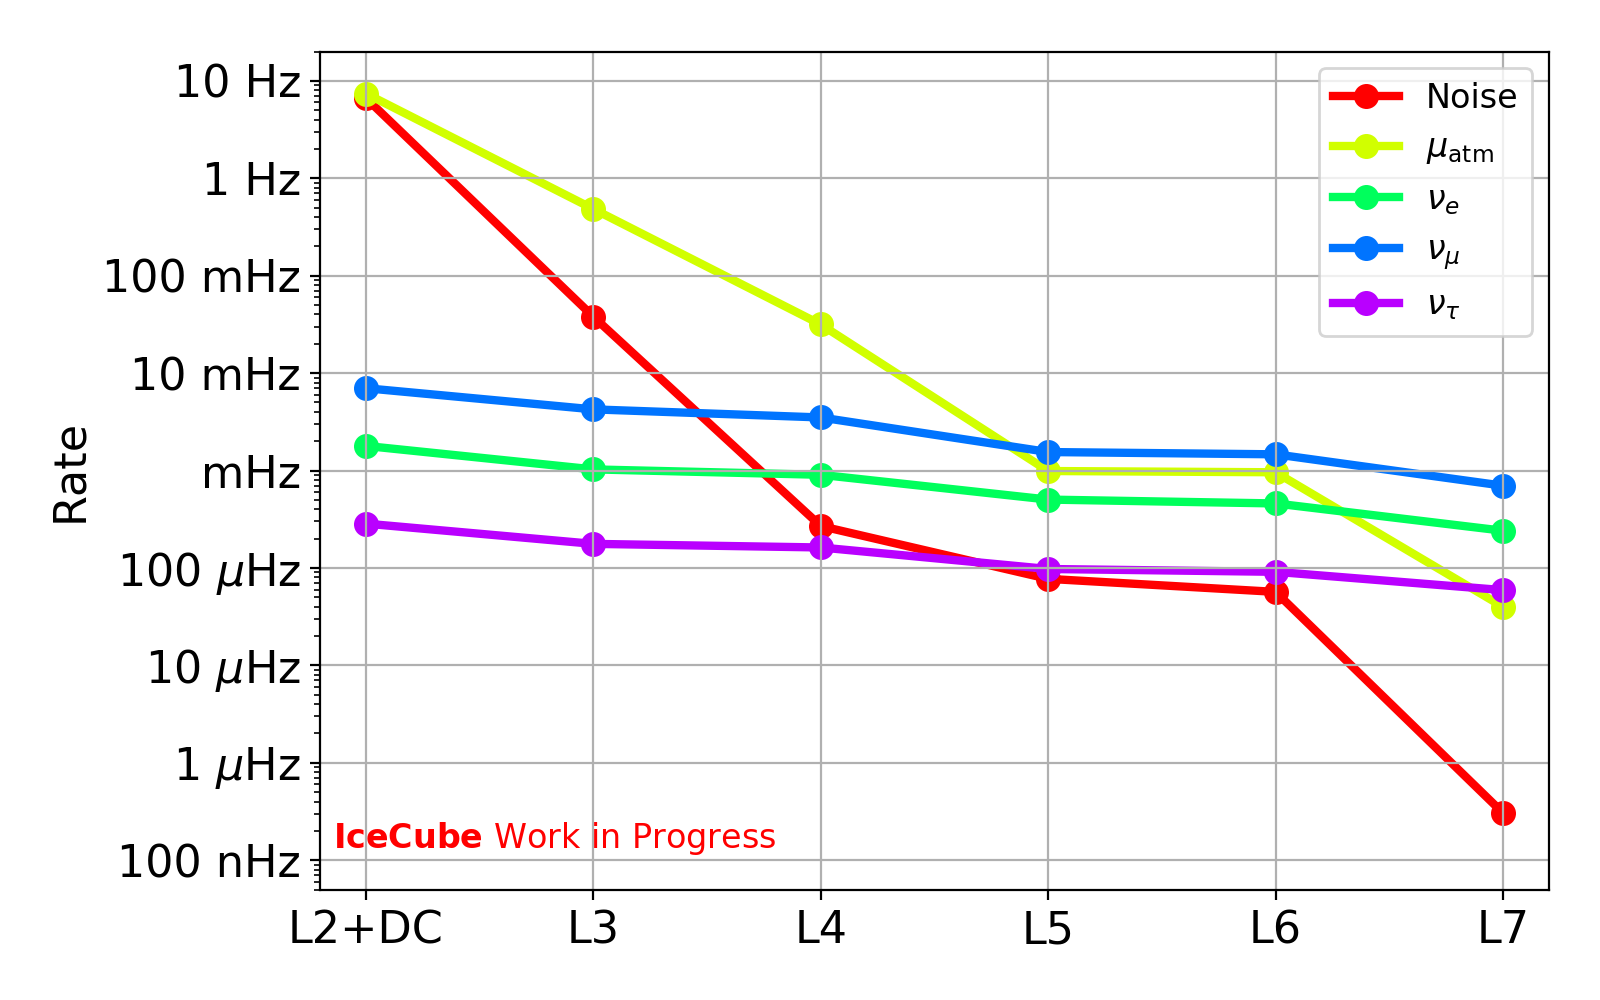
\includegraphics[width=.50\linewidth]{figures/OscNext_high_stats_event_selection_levels.png}
  \caption{Theoretical $\nu_{\mu}$ disappearance probability (left) and the rates of the IceCube neutrino sample selection steps (right).}
  \label{fig:oscnext_sample_and_phasespace}
\end{figure}

Observing the flux of atmospheric neutrinos above energies of $5\,$GeV, IceCube has the ability to measure $U_{\mu3}$, $U_{\tau3}$, and $\Delta m^{2}_{32}$. For this purpose, an event selection was developed that reduces atmospheric muon and noise contamination down to sub-percent level. \cref{fig:oscnext_sample_and_phasespace} shows the theoretical $\nu_{\mu}$ disappearance probability (left) and the rates at the different sample selection steps (right). IceCube is well suited to measure the effect of atmospheric neutrino oscillations that mainly occur in the 10-50\,GeV region. By measuring the relative fluxes of neutrino flavors as a function of their reconstructed energies and arrival directions (which can be related to the cosine of the incoming zenith angle), the parameters governing the oscillation pattern shown in \cref{fig:oscnext_sample_and_phasespace} can be measured. The flavor of the interacting neutrinos is inferred from the topology of the events, splitting the sample in track- and cascade-like parts. The analysis is performed using a binned maximum likelihood estimation to compare the data to MC simulation for a specific hypothesis. \cref{fig:oscnext_oscillations_results} shows the latest results of the 8 year IceCube DeepCore neutrino oscillation analysis using the golden (sub-)sample which constrained the atmospheric neutrino mixing parameters to be $\sin^2\theta_{23} = 0.505^{+0.051}_{-0.050}$ and $\Delta m^2_{32} = 2.41\pm0.084 \times 10^{-3}\mathrm{eV}^2$, assuming a normal mass ordering. Additionally shown is the expected sensitivity using the full statistics sample and the latest results from other experiments.

\begin{figure}[h!]
  \centering
  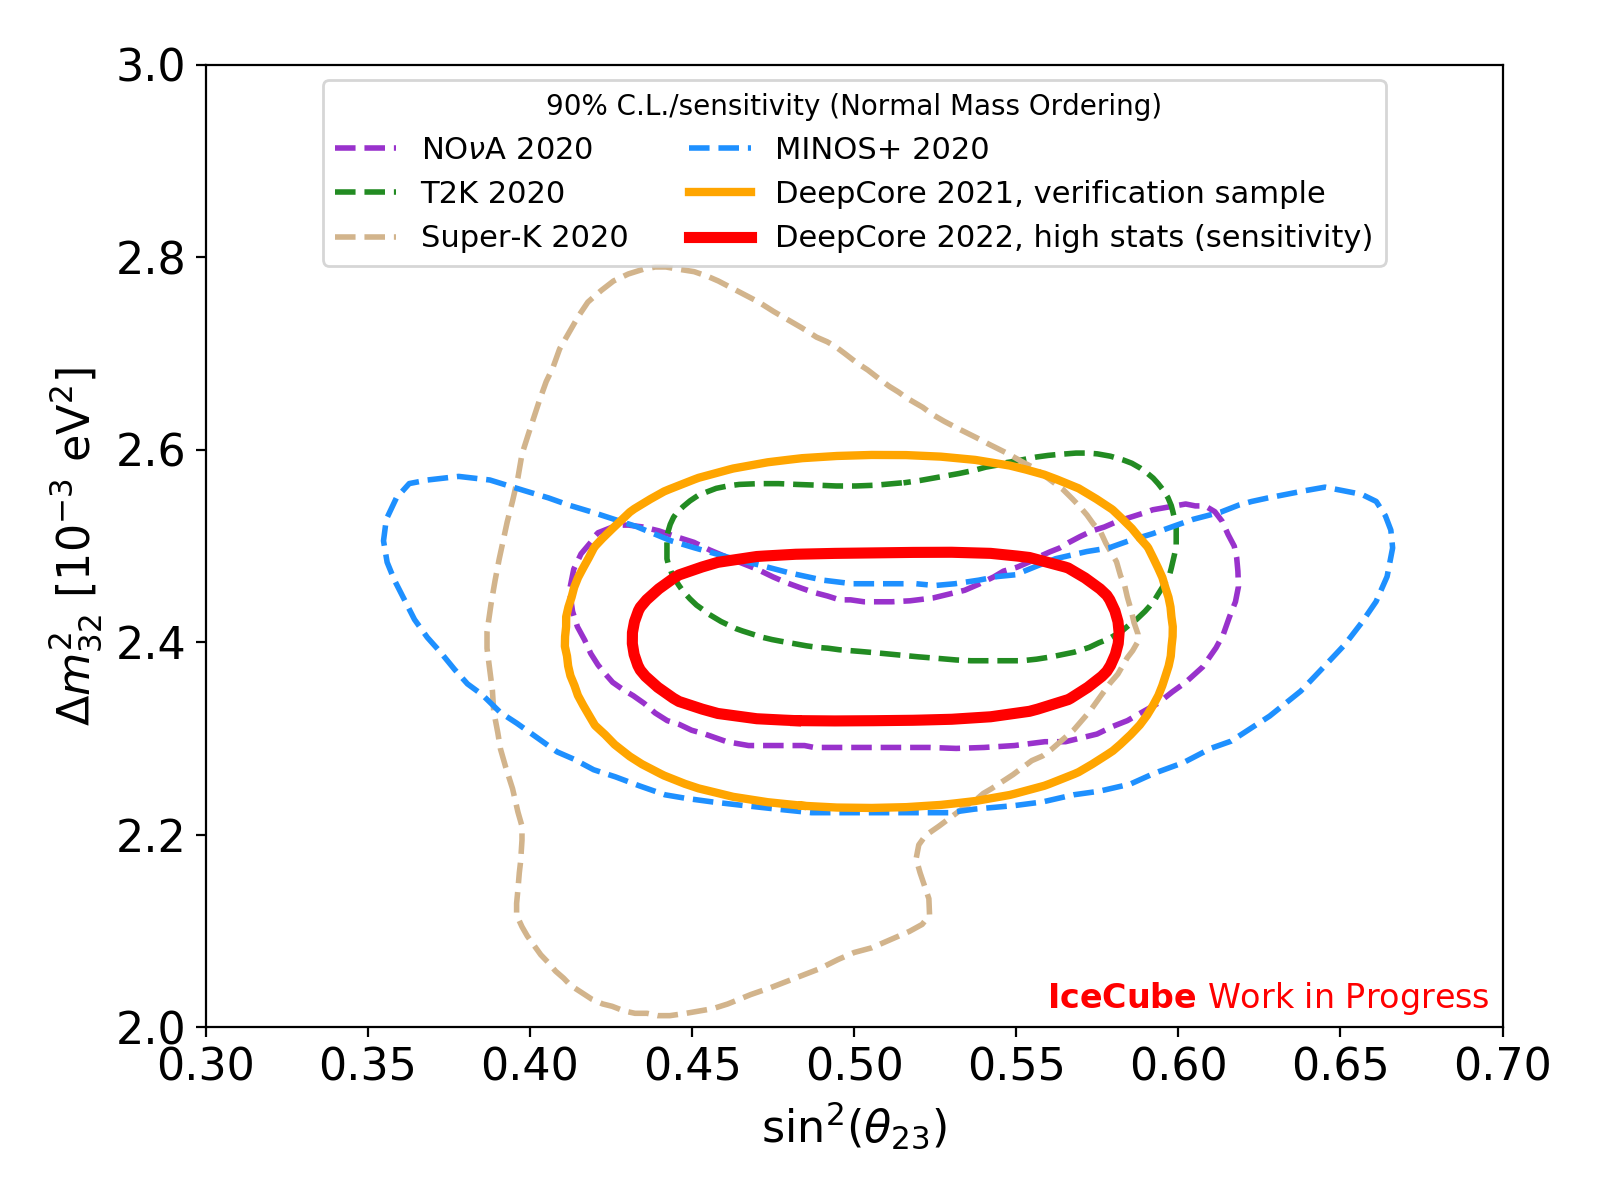
\includegraphics[height=0.4\linewidth]{figures/OscNext_numu_disappearance_sensitivity_public_v2.png}
  \caption{Latest results and expected sensitivity of IceCube Deepcore atmospheric neutrino oscillation analylsis.}
  \label{fig:oscnext_oscillations_results}
\end{figure}

\vspace{-0.5cm}
\section{Heavy neutral lepton search}

To incorporate the HNL into the original model, an additional heavy mass state and a sterile flavor state are added, turning the mixing relation into $\ket{\nu_\alpha} = \sum_kU^{4x4*}_{\alpha k}\ket{\nu_k}$, with $\alpha=e,\mu,\tau,s$ and $k=1,2,3,4$ and $U^{4x4}_{\alpha k}$ now being the extended 4x4 mixing matrix. $\nu_s$ is a SM, right-handed singlet fermion and therefore not charged under the SM gauge groups. If the mass of the HNL is in the $\sim$\,GeV region, it's production is kinematically accessible at atmospheric neutrino energies ($10-100$\,GeV) and the decay will happen to SM particles. Because of its singlet property, its only way of interaction is through the weak interaction, inherited from the left-handed neutrinos via mixing \cite{Coloma:2020lgy}. The goal of this work is to (first) probe the less constrained $|U_{\tau4}^2|$ mixing parameter, defining the $\tau$-sterile mixing space as shown in \cref{fig:hnl_limits_and_decay_widths}. Because of the phenomenon of neutrino oscillations, a significant part of the purely $\nu_{\mu/e}$ atmospheric neutrino flux oscillates into $\nu_\tau$ until it reaches the IceCube detector. The $\nu_\tau$ can interact in the ice, producing the new, heavy mass state in an up-scattering process, which itself travels for a certain distance and then decays into lighter SM particles. \cref{fig:hnl_limits_and_decay_widths} (right) shows the individual and combined decay widths to the SM particles. The production and the decay both produce a cascade-like light deposition and if the distance between the two is large enough and the energies are sufficient, it can produce a double-cascade-like light deposition. An example of this unique event topology is shown in \cref{fig:low_energy_eventviews}. We use the same event selection as was used for the neutrino oscillation analysis described in \cref{sec:neutrino_oscillations}. It was developed to select events in IceCube DeepCore targeting atmospheric neutrinos and rejecting muons and noise, but since the HNL events are produced from the atmospheric neutrino flux the event energies are very similar and starting from this selection is a valid first approach.

\begin{figure}[h!]
  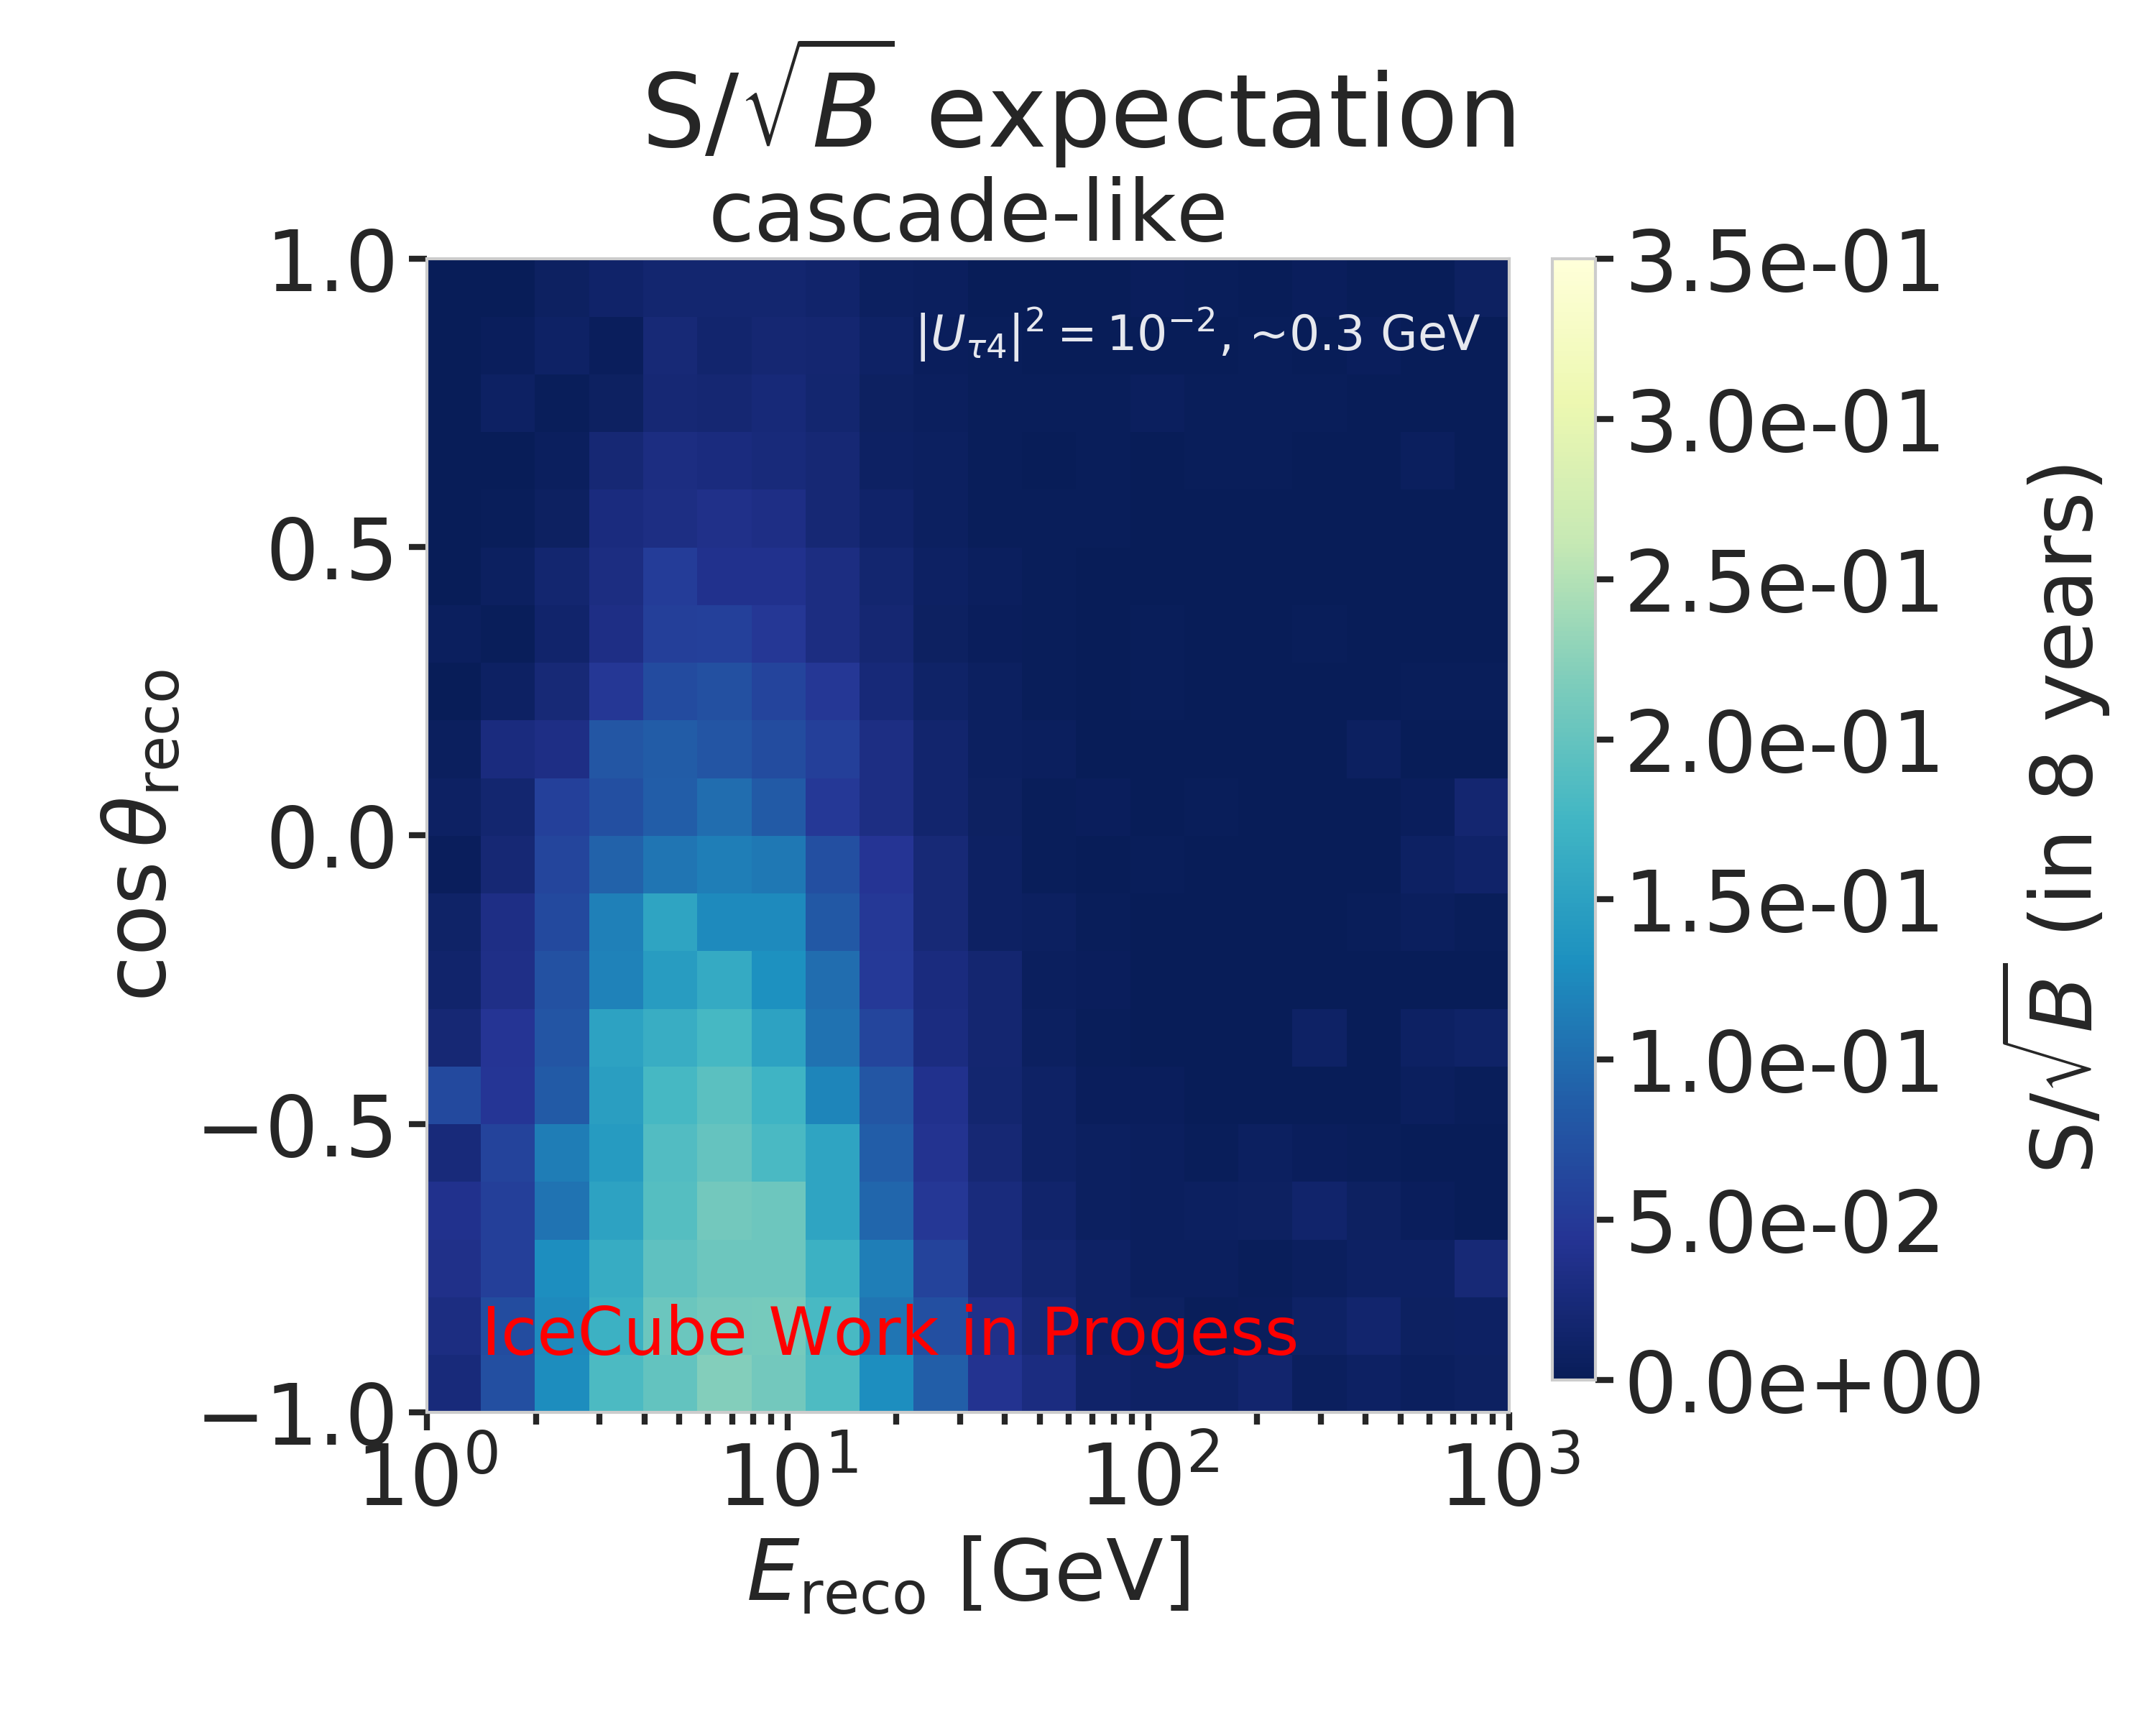
\includegraphics[height=0.4\linewidth]{figures/2_d_S_over_sqrt(B)_taupede_reco_energy_taupede_reco_coszen_around_0.3_GeV_new.png}
  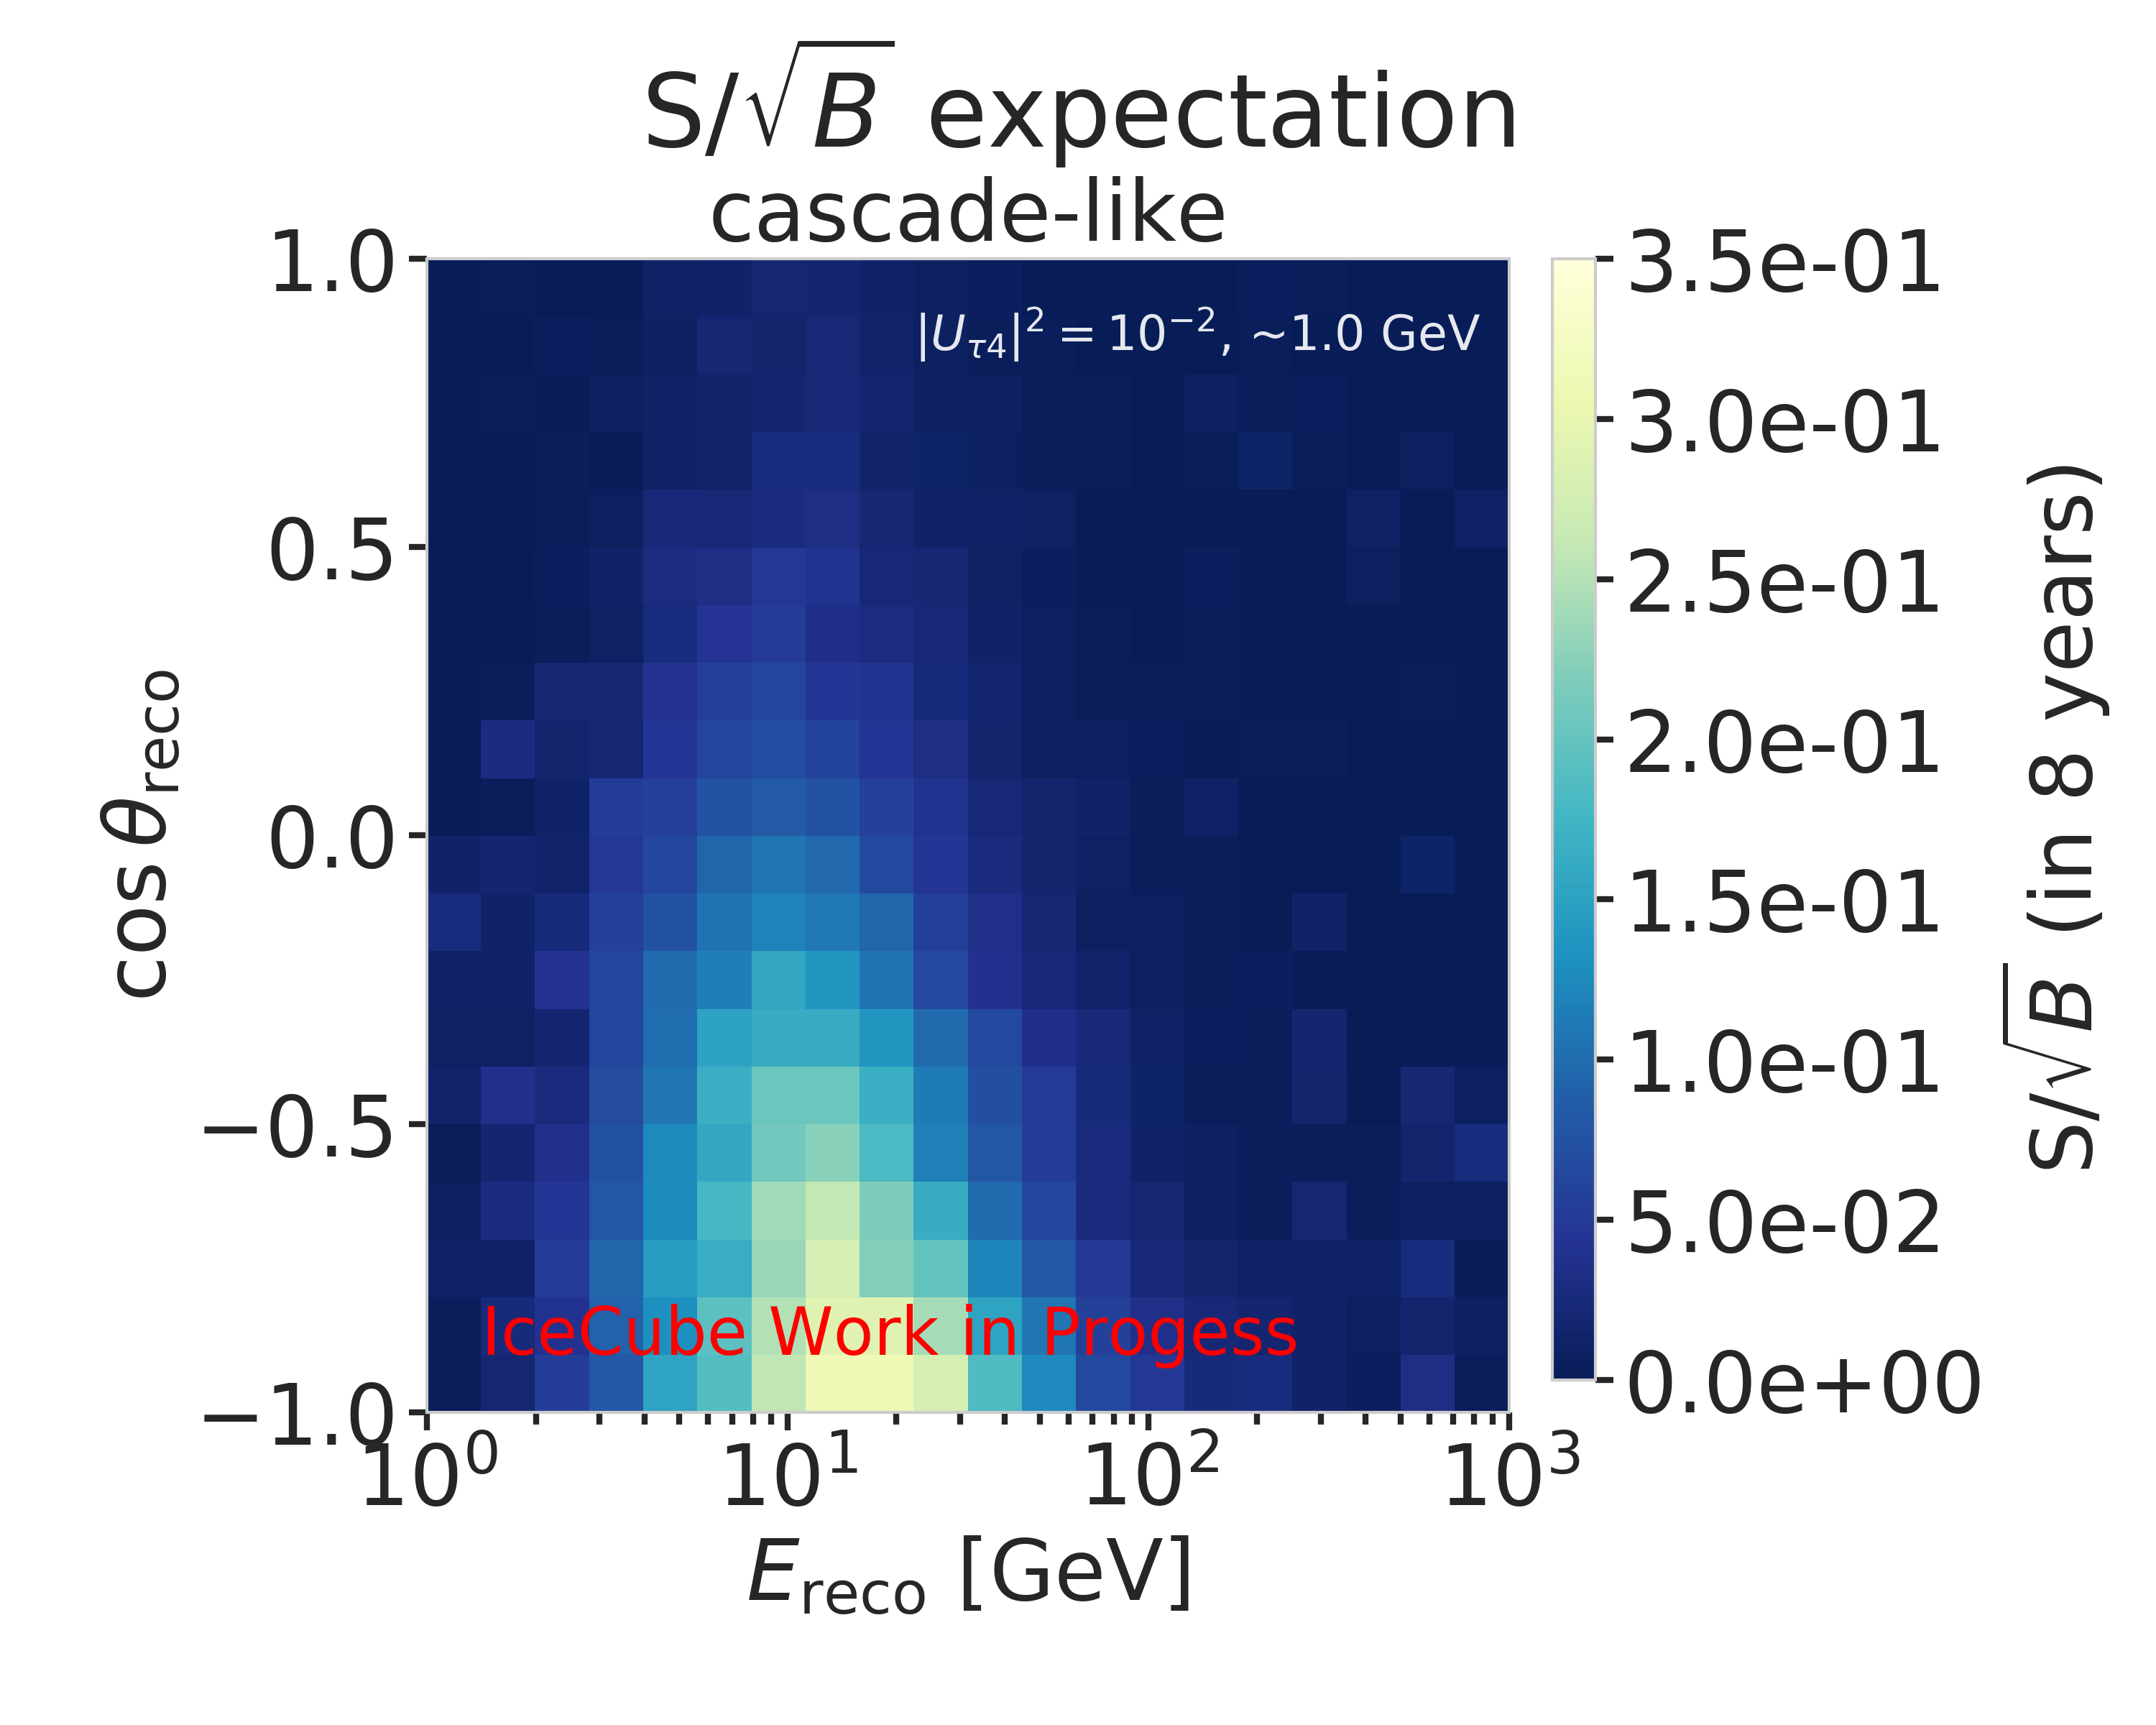
\includegraphics[height=0.4\linewidth]{figures/2_d_S_over_sqrt(B)_taupede_reco_energy_taupede_reco_coszen_around_1.0_GeV_new.png}
  \caption{Signal (HNL) over squre root of background (SM) in the cascade-like channel using the standard neutrino oscillation analysis binning for HNL masses of 0.3\,GeV (left) and 1.0\,GeV (right) and a mixing of $|U_{\tau4}^2|=10^{-2}$.}
  \label{fig:s_over_sqrt_B_HNL}
\end{figure}

The original analysis idea is to apply a specifically tailored reconstruction, assuming a double-cascade hypothesis, and then selecting them using a boosted decision tree (BDT) method, using the reconstructed double-cascade parameters as input. As outlined by \cite{Coloma:2017ppo}, isolating a double-cascade signal region should lead to strong constraints in the tested mixing-mass space, but it turns out that isolation a pure signal region is a more challenging task than expected. The main problem is that many of the SM neutrino interactions look very similar to the double-cascade events because the energies are generally very low, which results in very few photons being emitted and because of the sparsity of the detector only a fraction of those are detected. For the double-cascade events the energy distribution of the second cascade is especially low, because a part of the energy is oftentimes being carried away by the invisible neutrino. As a result, most of the HNL events look like single cascades. On top of that, the total HNL rate is much smaller than the SM neutrino rate ($S/B\sim O(10^{-4})$). Since this simple cut\&count analysis approach does not work, a more sophisticated principle is envisioned. Similar to the standard neutrino oscillation analysis, the events will be seperated in multiple particle identification (PID) bins as well as bins in other reconstructed quantities. The exact binning scheme is not defined yet, but the idea is to use the shape of HNL signal distributions on top of the SM backgrounds in cascade/track/double-cascade bins to constrain the mixing parameter. \cref{fig:s_over_sqrt_B_HNL} shows the signal over square root of background distribution in the (oscillation analysis) cascade-like PID bin. Using this binning, which was not optimized for the HNL search, the observed signal already looks promising.

\footnotesize
\bibliographystyle{JHEP}
\bibliography{MyBibFile}


\end{document}
